\section{Trådløs kommunikation gennem bluetooth}
\textit{I dette afsnit gennemgår design, implementering og test af systemets trådløse kommunikation mellem de to benyttede MCUer.}

\subsection{Design}
Systemet vil involvere to MCUer, henholdsvis en GAP central og en GAP peripheral. Begge enheder vil have påført et BLE modul, således dataoverførslen mellem enhederne vil foregå gennem brug af BLE. Denne dataoverførsel mellem MCUerne er illustreret som pseudokode på \figref{fig:blue_pseudo}. 

\begin{figure}[H]
	\centering
	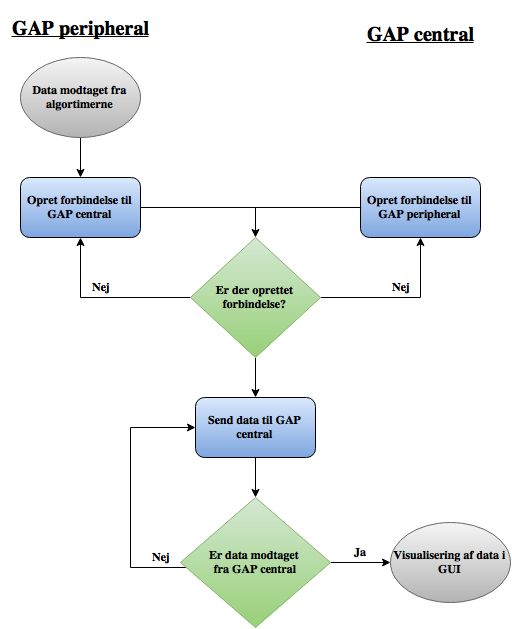
\includegraphics[scale=0.5]{figures/bProblemloesning/blue_pseudo.png}
	\caption{Illustration af den trådløse kommunikation og dataoverførsel mellem GAP central og GAP peripheral. Indledningsvis forsøges det at oprette forbindelse mellem enhederne, hvorefter dataoverførslen finder sted. Ved fuldendt dataoverførsel bliver BLE modulet for de to enheder slukket/sat i dvale.}
	\label{fig:blue_pseudo}
\end{figure}

Det er kodningen som er bestemmende for hvorvidt en MCU vil fungere som GAP central eller peripheral i et kredsløb. Den enhed som initialiseres til GAP central skal modtage data fra den anden enhed. Ydermere skal GAP central overføre denne data til en computer gennem en USB port, således visualisering i et GUI er muligt. \newline
Førend en dataoverførsel er mulig, er det nødvendigt at der er skabt en forbindelse mellem de to enheder, hvilket ligeledes fremgår af \figref{fig:blue_pseudo}. Hvis ikke det lykkes at oprette forbindelse, gentages denne procedure. Når der er etableret forbindelse mellem enhederne overføres dataene, som har været gemt i flash hukommelsen på PSoC 4200M. Ydermere vil systemet ikke fortsætte til næste element i pseudokoden, medmindre dataoverførslen har været succesfuld.  

\subsection{Implementering}
GAP peripheral er den MCU som er ansvarlig for dataopsamling, lagring af data og afsendelse af data til GAP central. Gap peripheral vil dermed benytte et samarbejde mellem PSoC 4200M og EZ-BLE. Konfigureringen af henholdsvis GAP central og GAP peripheral udføres i PSoC Creator, hvor ’Topdesign’ af EZ-BLE modulerne er afgørende for deres rolle i kredsen. \newline
PSoc 4200M på GAP peripheral vil blive konfigureret således dataoverførslen vil blive ført mod EZ-BLE. Denne konfigurering udføres ved at initialisere de pågældende pins for PSoC 4200M og EZ-BLE i pindesign i PSoC Creator. Port P3[0] bliver benyttet til UART:rx og port P3[1] til UART:tx. Ydermere konfigureres EZ-BLE modulet til at benytte P1[4] til UART:rx og port P1[5] til UART:tx. Disse konfigureringer sikrer at der forekommer en dataoverførsel fra PSoC 4200M og videre til EZ-BLE, hvorfra dataene kan sendes til GAP central. \citep{Semiconductor20164200M} \newline
GAP skal central konfigureres, således denne kan modtage data og herefter overføre dette til en computer gennem USB porten. For at sikre disse handlinger, benyttes samme pins til UART mellem EZ-BLE og PSoC 4200M. Ydermere benyttes port P7[0] til UART:rx og port P7[1] til UART:tx. Dermed er det muligt at overføre datene fra PSoC LP5 til en computer. 

Det fremgår af \figref{fig:blue_pseudo}, at BLE modulerne skal sættes i dvale/slukkes når dataoverførslen er fuldendt. Derfor vil C kodning af BLE modulerne medvirke til, at denne handling er mulig. DER SKAL NOK SKRIVER MERE HERTIL NÅR VI VED HVORDAN VI BENYTTER POWERMODES.


\subsection{Test}
